% !TEX root = Technologierecherche.tex
\section{Lenkung}
\subsection{Knicklenkung}
-Die Hinterachse volgt immer der gleichen Spur wie die Vorderachse.\\
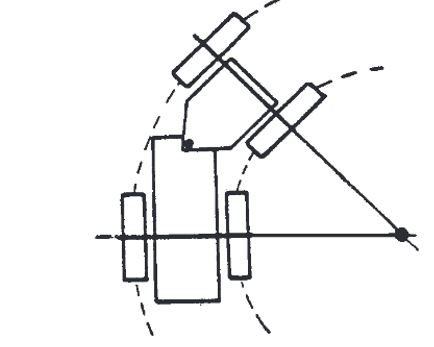
\includegraphics[width=0.5\textwidth]{Images/Knicklenkung.JPG}
\subsection{Achsschellenlenkung}
-Die Standfestigkeit wird auch bei vollem Lenkeinschlag nicht beeinträchtigt.\\
-Heutige zweiachsige PWS und Nutzfahrzeuge sind fast alle mit Achsschellenlenkung gebaut.\\
-Das kurveninnere Rad ist stärker eingeschlagen als das kurvenäussere.\\
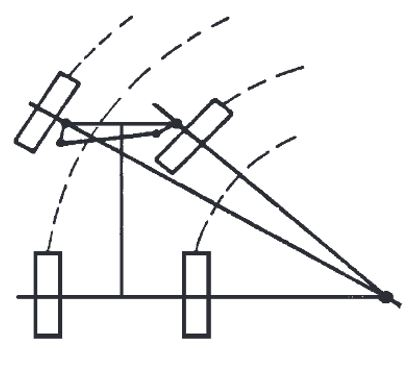
\includegraphics[width=0.5\textwidth]{Images/Achsschellenlenkung.JPG}
\subsubsection{Lenktrapez}
-Ermöglicht unterschiedliche Einschlagwinkel der Vorderräder.\\
-Ermöglicht einfaches einstellen eines Spurwinkels.\\
-Zur Berechnung von Lenktrapezen gibt es vorgefertigte EXEL Tabellen im Web.\\
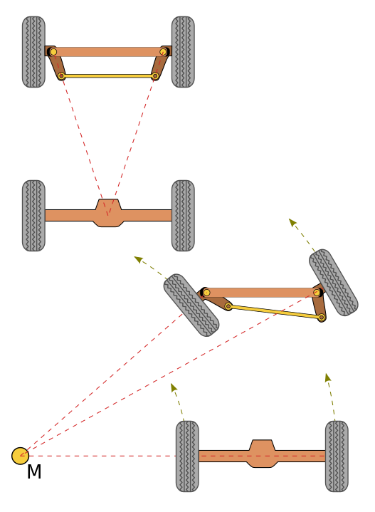
\includegraphics[width=0.5\textwidth]{Images/Lenktrapez.png}

